\section{Sunquakes}
\subsection{An Introduction to Sunquakes}
%Chronological soft intro; use some of the lit review,
%making sure to emphasize the connection to solar flares;Look at early papers predicting sunquakes(Wolff 70s and Kosovichev and Zharkova);the importance of sunquakes



Sunquakes are caused by energy and momentum impacting the lower solar atmosphere. During a solar flare, energy is transported from high up in the solar atmosphere down to lower regions. If a sufficient amount of energy impacts the lowest atmospheric layer, then acoustic waves are produced which propagate into sub-surface layers of the Sun (see figure \ref{sunquake-cartoon}a). As acoustic wavefronts travel into the interior they encounter layers of increasing density causing refraction back toward the solar surface (see figure \ref{sunquake-cartoon}b). At which point, waves can be observed as circular formations in the surface plasma, expanding outward from a point of origin.         


\begin{figure}\label{sunquake-cartoon}
  \begin{center}
  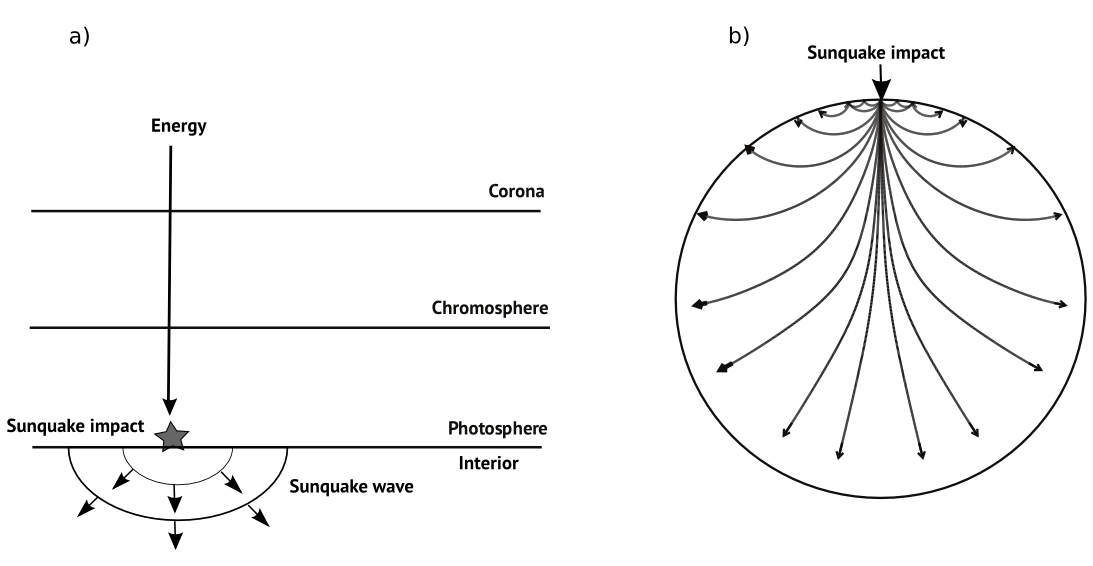
\includegraphics[width=0.40\textwidth]{sunquake-cartoon}
  \end{center}
  \caption{Sunquake cartoon: a) Shows a basic picture of sunquake production. Energy moves down through the solar atmosphere impacting the photosphere and generating a sunquake. b) Shows acoustic wavefronts propagating into the interior of the Sun. Wavefronts refract back toward the surface as they encounter increasingly dense sub-surface layers. Waves reaching the surface disturb material in a pattern resembling ripples in a pond.}
\end{figure}

One can consider a sunquake to be an observable signature of energy being deposited by a solar flare. The possability that solar flares could cause acoustic waves inside the Sun was originally put forward by \citep{1972ApJ...176..833W}. Wolff suggested that........ 

This idea was built upon by \cite{1995ESASP.376b.341K}, who showed theoretically that acoustic waves in the solar interior could be generated by a large solar flare. This research also showed that these acoustic waves may be detectable. A year later and the prediction of detection came to fruition when \cite{1998Natur.393..317K} made the first observation of a sunquake during an X class solar flare on July the 9th 1996. Their observations came from the Solar and Heliospheric Observatory (SOHO) via the Michelson Doppler Imager (MDI) which images the movement on material by analysing shifts in wavelength of the captured light. 

\ref{mdiquake96}

\begin{figure}\label{mdiquake96}
  \begin{center}
  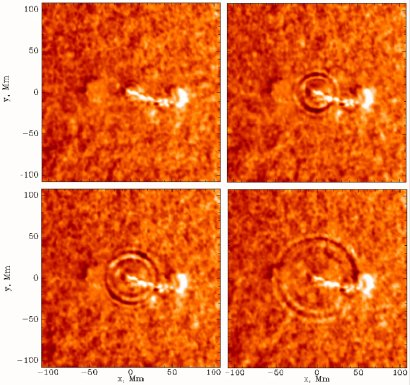
\includegraphics[width=0.40\textwidth]{soho-mdi-quake-96}
  \end{center}
  \caption{\cite{1998Natur.393..317K} produced SOHO MDI Dopplergrams from the 1996 July 9th, X class solar flare showing the sunquake evolving over time. Each frame relates to a $####s$ progression in time. The sunquake expands outward from it's seismic epicenter to a radial distance of $####Mm$ with a wave amplitude of $###km$ . Wavefronts accelerate over time, propagating with an average velocity of $###km.s^{-1}$ }
\end{figure}

The seismic wave propagated through the photosphere, to a distance of $1.2\times10^{8}$ metres from it's point of origin at an increasing velocity of $30$ to $100 km.s^{-1}$. Kosovichev and Zharkova commented that observed Dopplergrams revealed strong mass flows both upward and downward during the impulsive phase of the flare, of which the maximum flow velocity occurred around 1 minute later. The other interesting comment from this article was that this time delay was consistent with the thick target model of solar flares, in that an incident particle beam heats the cooler chromosphere causing a shock front which travels downward, impacting the photosphere, as it stands, this idea is yet to be proven. This article also mentions the use of seismograms to track the sunquake, constructed by remapping Doppler images into polar coordinates centered on the point of initial velocity impulse, then applying a Fourier transform with respect to the azimuthal angle. The seismogram will produce a set of ridges with a positive slope, in-fact the plot produced with this technique showed how the wave packet accelerates over time.      
%%%%%%%%%%%%%%%%%%%%%%%%%%%%%%%%%%%%%%%%%%%%%%%%%%
%old report content


%%%%%%%%%%%%%%%Sunquakes%%%%%%%%%%%%%%%%%%%%%%%%%%%%%%%%%%%%%%%%
\subsection{Sunquakes}\label{SQK}
Sunquakes are the propagation of acoustic waves in the sub-photosphere, observed in Dopplergrams as concentric oscillations of photospheric material. During a solar flare, energy is some how transported from the reconnection site of the magnetic field in the corona, down through the transition region and chromosphere, impacting the photosphere. This energy is deposited at the photosphere in such a way that an acoustic wave is produced which travels into the interior of the sun until refracting back toward the surface, at which point material can be observed as moving toward the observer in a circular pattern resembling pond ripples. 

%%%%%%%%%%%%%%%%%%%%%%%%%%55literature review%%%%%%%%%%%%%%%%%%%%%%%%
\subsubsection{Literature Review}
This chronological review of literature concerning sunquakes is not the entirety of the research done by the author of this report. More, it is a collection of papers and reviews that seem of importance in the grand scheme of the area of research.   \\


\citep{1972ApJ...176..833W}. Since Wolff's paper it took around twenty years until the first observation of an acoustic wave, or sunquake, was realised. \cite{1998Natur.393..317K} observed an acoustic oscillation of the solar photosphere with an amplitude of three kilometers in altitude, caused by an X-ray flare that occurred in July 1996. The seismic wave propagated through the photosphere, to a distance of $1.2\times10^{8}$ metres from it's point of origin at an increasing velocity of $30$ to $100 km.s^{-1}$. Kosovichev and Zharkova commented that observed Dopplergrams revealed strong mass flows both upward and downward during the impulsive phase of the flare, of which the maximum flow velocity occurred around 1 minute later. The other interesting comment from this article was that this time delay was consistent with the thick target model of solar flares, in that an incident particle beam heats the cooler chromosphere causing a shock front which travels downward, impacting the photosphere, as it stands, this idea is yet to be proven. This article also mentions the use of seismograms to track the sunquake, constructed by remapping Doppler images into polar coordinates centered on the point of initial velocity impulse, then applying a Fourier transform with respect to the azimuthal angle. The seismogram will produce a set of ridges with a positive slope, in-fact the plot produced with this technique showed how the wave packet accelerates over time. \\


\cite{1999ApJ...513L.143D} pioneered the use of helioseismic holography to produce seismic images of the solar flare of July 1996 reported to have a sunquake by Kosovichev and Zharkova \citep{1998Natur.393..317K}. Time series egression-power maps at 3.5 and 6 mHz were computed with a 2 mHz bandwidth. It was found that the most powerful acoustic power frequency associated with the flare is centred at 3.5 mHz but has a large signal to noise ratio. Whereas the 6 mHz range has a much lower ambient noise, therefore producing a better rendering of the seismicity of the flare. It is now standard practice to use the 6 mHz range for helioseismic holographic calculations of egression-power. \\


The first simulations of sunquakes came to fruition in 2000 when \cite{2000AcA....50..405M} ran 2D numerical simulations of sunquake waves in the sub-photosphere based on Euler's compressible fluid dynamics equations. Magnetic fields were neglected. The model included two layers of the atmosphere with the photosphere at a constant temperature and the sub-photosphere increasing in temperature linearly with depth. The point of origin of the sunquake was placed just below the photosphere. The simulation produced an initial pulse of enhanced pressure, just below the photosphere in the sub-photosphere, which becomes an acoustic wave. The wave interacts with the photosphere causing perturbations which would be observed as sunquakes. The model reproduced wave signatures and wave acceleration (from epicenter) profiles associated with the observed properties of sunquakes, and also found seismic waves to be dispersive and non-linear.\\

\cite{2001ApJ...550L.105K} report observations of magnetic transients on the photosphere during a solar flare, where by impulsive changes in magnetic field strength were observed. These magnetic transients were shown to approximately correlate in time and space with impulsive increases in plasma velocity and emission intensity. The author puts forward the idea that the observed transients are caused by beams of energetic particles reaching the photosphere.\\   


Inevitably, a few years later another set of simulation data was reported, this time looking into any similarities between sunquakes and water waves. This was probably due to the resemblance of sunquake Doppler images to the appearance of ripples caused by the dropping of a stone in a pond. The model put forward by \cite{2003SoPh..218..227P} simulated seismic waves at the surface of the convective zone using incompressible fluid dynamics, the same method for simulating water waves. It was noted by the author that incompressible fluid dynamics is not realistic in terms of sunquakes, due to acoustic waves in the convective zone being dominated by compressible p - modes. Also, this highlighted the fundamental difference in the physics of water waves and sunquakes. The reason sunquakes were studied in this way was to pave the way for more complicated, compressible fluid models. These simulations were able to produce the ring waves observed on the surface of the convection zone during a sunquake. The acoustic waves were shown to disperse strongly, leading to a quadratic time-distance relationship, implying a constant radial acceleration of wave crests. However, observations show that not only do the crests and troughs of the acoustic waves accelerate but so does the entire wave packet, this is where this particular model failed.\\


\cite{2005ApJ...630.1168D} detected acoustic waves associated with the solar flares on October 28th and 29th AR10486 and using helioseismic holography, calculated egression maps to image the seismic sources. Egression-power (6mHz with 2mHz bandwidth) maps revealed compact acoustic sources that were well aligned with hard X-ray signatures associated with the footpoints of coronal loops. This suggested a link between accelerated particles during the flare and a movement of material in the chromosphere or photosphere underneath the footpoints. There was also evidence of high energy protons entering the chromosphere in the vicinity of the acoustic sources. Emission associated with the D1 line of neutral sodium observed from the 29th of October flare suggested condensation of chromospheric material at the onset of the flare. The Global Oscillation Network Group (GONG) also observed the events and intensity data showed enhanced radiative emission with an impulsive profile aligned in space and time with the seismic source. As a result of this wealth of observational data, this paper reported a number of conclusions. The energy needed to stimulate the propagation of an acoustic wave in the sub-photosphere is a very small fraction of that released by the flare. A plot showing intensity over time showed that the flares had a highly impulsive phase. The authors put forward the idea that the existence of an acoustic source, relies more on how suddenly the energy is released rather than the energy budget of the flare. There was evidence of energetic chromospheric condensations above the seismic source. The authors stress the importance of high-energy protons reaching the lower altitudes of the chromosphere and even the photosphere where the thick target is more massive compared to the upper chromosphere where electrons deposit their energy. Due to the extra mass in the lower chromosphere and photosphere, a greater fraction of the protons energy can be used to create an acoustic wave.  \\


Between 2003 and 2005, \cite{2006SoPh..238....1K} observed four solar flares with associated helioseismic waves using SOHO. Comparing X-ray fluxes from RHESSI data. Again HXR sources were found to align well with sunquake points of origin which is indicative of high-energy electrons producing compression waves of sufficient strength to generate the sunquake. Data revealed new properties of sunquakes in the anisotropy of acoustic waves with the direction of propagation varying the amplitude. The anisotropy of these waves challenges theoretical models \citep{2000AcA....50..405M,2003SoPh..218..227P, 2005SoPh..232....1P} because they assumed a concentrated Gaussian impulse which is normal to the photosphere predicting an isotropic acoustic response. It was postulated that anisotropy could be due to a sequential release of energy + complex magnetic field geometry dictating the flow of plasma and direction of accelerated particles. The most interesting point in the conclusion pointed to the possibility that anisotropy could be caused by constructive interference of multiple flare energy impacts, distributed spatially and temporally. Such moving sources could be caused by consecutive events at the footpoints of neighbouring flux tubes. Waves propagating in the same direction as the expansion of flare ribbons would be evidence for this. The author also remarked about waves travelling through sunspot regions that are left undistorted. P-modes are usually damped by around 50\% in sunspots, which is attributed to energy escaping along the more radial magnetic field lines as MHD waves, whereas sunquakes seem largely unaffected. This is probably due to sunquakes propagating into the deep interior of the Sun rather than travelling horizontally across the surface. \\


\cite{2006SoPh..239..113D} observe a sunquake associated with an M class white light flare (WLF). The spatial correlation of white-light enhancement (WLE) and sunquake pointed at the first evidence that seismic waves are generated by heating of the lower photosphere. Sudden white light enhancement of the photosphere indicates an energy deposition via heating great enough to contribute to the observed emission released during the flare. In summary, the authors found: M class flares can have more associated seismicity than higher energy flares; the flare they studied had a strong spatial and temporal correlation between the sunquake and white light emission enhancement, which is explained by relating acoustic waves with sudden heating of the low photosphere; co-spatial WL and sunquake sources, where there was no evidence of energetic protons, adds weight to radiative backwarming as the progenitor of acoustic activity. The acoustic source was spatially and temporally aligned with a magnetic transient suggesting that magnetic forces may contribute to the seismic emission, a theory first mentioned by \cite{2001ApJ...550L.105K}. \\

The paper by \cite{2007MNRAS.374.1155M} reported that the sunquake was co-spatial with HXR and WLE along the penumbral neutral line. The WLE was estimated as having energy $E_{WL}=2.0\times10^{23}J$. The sunquake was estimated to have $E_{SQ}\sim4\times10^{20}J$. The energy available in the WL emission was 500 times greater than the sunquake energy. Again, the co-spatial nature of WLE and Sunquake point to the radiative backwarming progenitor for local seismicity, where by the photosphere is heated by Balmer and Paschen continuum radiation from the lower chromosphere. There was no evidence of protons.  \\

\cite{2007ApJ...664..573Z} detected three acoustic sources (S1, S2 \& S3) in MDI Dopplergrams using TD diagrams \ref{TD}. TD diagram derived start times and momenta were compared to that delivered by high-energy particles associated with HXR and $\gamma$-ray emission, as well as hydrodynamic shocks caused by these particles. S2 and S3 had signatures of HXR and $\gamma$-rays resulting from energetic protons, which could deliver sufficient momentum to cause shocks deep enough in the atmosphere to propagate down a short distance to the photosphere, whereas a high energy electron beam would not have enough momentum. S1 seemed to be associated with an electron beam.\\

\cite{2007SoPh..245..121M}, observed a sunquake associated with an M class flare. HXR, WLE and seismic sources were co-spatial, reinforcing the idea that sunquakes are produced by radiative backwarming of the photosphere by the chromospheric source of the continuum emission. 


\cite{2008ASPC..383..221H} explains the magnetic field variation (McClymont Jerk) progenitor, which could result from  a coronal mass ejection during an eruptive flare.  \\

\cite{2008SoPh..251..627L} makes the first real effort to list and explain all the current possible sunquake progenitors:
Chromospheric shocks caused by sudden thick target heating in the upper and middle chromosphere; wave-mechanical transients driven by heating of the photosphere; Lorentz-force transients resulting from magnetic reconnection in the corona. The author concludes that magnetic measurements after the impulsive phase of the flare cannot be entirely trusted due to molecular contamination of the sunspot spectrum and that any one model of sunquake generator is considered to be an over-simplification. \\

At the same time, \cite{2008SoPh..251..641Z} was also reviewing the possible progenitors of sunquakes. Starting by listing observed properties of sunquakes:
\begin{itemize}
\item Always associated with shocks propagating downward observed in Dopplergrams.
\item There can be many simultaneous or delayed seismic sources in the same flare.
\item The majority of sunquakes are anisotropic in appearance.
\item The majority of X class flares are seismically inactive. In high energy flares that do have sunquakes, only a very small fraction (a few thousands of a percent) of the flare's energy is needed to generate the acoustic waves. 
\item M class flares with large HXR flux seem to be the most seismically active cases.
\item Sunquakes associated with M class flares are often accompanied by WLE.
\item Seismic sources are regularly co-spatial with HXR and sometimes $\gamma$-ray emission in the footpoints of coronal magnetic loops, which is an indicator of high energy particles.
\item The previous point hints at acoustic waves being generated by impulsive heating during the onset of the flare, probably caused by hydrodynamic pressure response due to thermal dissipation of incident high energy particles.
\end{itemize}
The author then lists, explains and argues for or against a variety of different processes said to be possible contributors to the generations of seismic waves. The main conclusions drawn from this work are that the point of origin of sunquakes are usually associated with HXR emission and occasionally $\gamma$-rays in the footpoints of magnetic field loops. This points to accelerated high-energy particle beams, formed during X class flares with sunquakes, containing both electrons and protons being capable of transporting energy to the lower regions of the atmosphere. Energy deposited by the beams heats the atmosphere impulsively during the onset of the flare causing a hydrodynamic response propagate downward which impacts the photosphere generating the sunquake. M-class WLFs with associated seismicity are said be also generated by electron beams depositing energy into the chromosphere, which then heats the lower layers via radiative backwarming.\\

\cite{2008MNRAS.389.1905M} investigates the magnetic topological structure of a coronal magnetic field associated with seismicity. The motivation of which was to find out if the magnetic field can hinder the spread of sunquake waves from the epicenter of the seismic source, and if there is a particular magnetic field configuration that facilitates seismicity in the photosphere. The author concludes that the area of peak seismicity was shown to exist under a highly twisted magnetic field, therefore the photospheric impact was greatest where the magnetic field had large amounts of stored energy.\\   

\cite{2009MNRAS.395L..39M} analyses the magnetic field variation of the photosphere in many flares, looking for the 'McClymont Jerk' and any correlation with seismicity. The study finds that some flares with seismicity do not have a spatial and temporal correlation between sunquakes and magnetic transients. Some flares have magnetic transients and no seismicity, and some flares have a good co-spatial alignment of acoustic activity and magnetic variability. The author concludes that maybe the impulsiveness of the magnetic field variation could be important as to whether a sunquake is generated. Also, that at the time of the publication, the involvement of magnetic transients is unclear and more work needs to be done.

\cite{2011SSRv..158..451D}, presents a review of the current understanding of sunquakes, the mechanisms of generation and existing models. The author first lists what is known so far about sunquakes:

\begin{itemize}
\item They are unusual. The majority of flares do not generate seismic emission observable in the p-mode spectrum.
\item Only a tiny amount of the radiative flare energy is needed to generate a sunquake.
\item Sunquakes are the most compact seismic sources observed.
\item Relatively, sunquake emission is the most intense observed at high frequencies.
\item Impulsive WLFs generate the majority of sunquakes. 
\item Multiple seismic sources in the photosphere have been generated by flares simultaneously.
\item Sunquakes are produced frequently by flares with proton beams but also by flares without proton beams
\item Lorentz forces created by changing magnetic structures in active regions may have a part to play in facilitating the generation of sunquakes.
\end{itemize}

This is an extensive review, however these are the points that stood out as being of particular importance. The authors comment that in WLFs, the highest most impulsive concentrations of WLE generate sunquakes with the most efficiency. Of these compact events there is often similar features seen in both the seismic and WL kernels, that is, a bright inner core surrounded by an fainter asymmetric halo. The sunquake's point of origin is often located in the penumbra of a sunspot. If photospheric heating is responsible for generating the quake, then the $5-7$mHz acoustic power maps should look similar to intensity continuum power maps of the same band.\\
The current progenitors associated with this review:
\begin{itemize}
\item Explosive ablation of the chromosphere via high-energy electrons causes shocks. The argument against this idea is the heavy radiative losses that such a shock wave would encounter in the lowest regions of the atmosphere.  
\item Heating of the low photosphere observed as WLE, i.e., the radiative backwarming method.
\item Direct proton beam interaction: observed in some flares associated with sunquakes. However, not all seismically active flares exhibit proton beam signatures. 
\item Reconfiguration of coronal loops via a relaxation to lower altitude flux tubes. The change in magnetic field inclination at the footpoints drives the generation of Lorentz force transients that could cause a sunquake if the "McClymont jerk" is sudden enough.
\end{itemize}


\cite{2011ApJ...741L..35Z} report the observation of two seismic sources associated with a flare that erupts producing a coronal mass ejection (CME). This event is different to most sunquake observations because the seismic sources are not spatially or temporally aligned with HXR emission, meaning they are not associated with energy transport via high-energy particle beams; neither are they associated with white light emission, ruling out radiative backwarming. Instead the two seismic sources are located beneath a large magnetic structure called a sigmoid which indicate the existence of a flux rope. When the flux rope rises due to local magnetic reconfiguration the flare erupts leading to a two ribbon event. The authors raise the question as to how an erupting flux rope could possible cause the two observed quakes? Considering hydrodynamic shocks and magnetic restructuring as possible answers.\\
Hydrodynamic shocks caused by heating of the lower atmosphere by a small enough population of energetic particles not to generate sufficient HXR emission. These particles can be taken from the corona and separatrix jets and are filtered along arcade field lines until they wrap around the flux rope where they deposit their energy. During the eruption, the magnetic field above each seismic source undergoes an abrupt permanent reconfiguration. Over the strongest sunquake there is a definite observable change, whereas over the weaker sunquake the data is more challenging due to the field being in a constant, slower state of change. Both sources are located in penumbral regions, with relatively horizontal magnetic fields which is favourable for the magnetic jerk idea.\\


\cite{2011ApJ...739...70Z} develop an updated technique for identifying sunquakes from GONG data, comparing their findings to the same observations made with SOHO/MDI. Egression maps and TD diagrams are computed from both GONG and MDI data. They find that local helioseismology data derived from GONG is in good agreement with the same data from MDI, in that GONG is capable of capturing local seismic events. Processed GONG data however has a low signal to noise ratio when compared to MDI, which leads to trouble differentiating sunquake sources from sunspots in the egression maps. TD diagrams from GONG are in agreement with MDI regarding locations of sunquakes. The higher resolution data from MDI is able to produce a more detailed TD diagram than GONG, again because of noise and atmospheric turbulence experienced by the Earth based instrument. This work means that it is possible to investigate seismicity associated with flares that happened before MDI or SDO HMI observations existed.\\    



\cite{2012SoPh..277..317P} perform a statistical survey of WLfs with and without sunquakes. Of the sample of nine WL flares considered in this study, five had sunquakes and four did not. The authors present a summary of their results in list format:
\begin{itemize}
\item In seismically active WL flares, it was found that electron energy deposition occurs at a higher rate than in seismically quiet flares.
\item The area over which energy is deposited is approximately the same for the entire sample of flares
\item In flares with sunquakes, the WL kernel is less compact and has lower contrast than in flares without sunquakes.
\item A flare containing three footpoints had a seismic source that was co-temporal but not co-spatial with it's closest footpoint; and another source which was co-spatial and co-temporal (if errors are considered) with it's nearest footpoint.
\item Emission in HXR and WL are in good alignment in space and time, often being over the origin of a sunquake. HXR and WL emission of the highest contrast is not always associated with a sunquake. 
\item There is sufficient energy budget in all measured electron distributions to give up to seismic emission.
\end{itemize}

The main points to take away from this review are that a simple model of sunquake mechanism probably does not exist. The problem seems to be that the solar atmosphere is a very dynamic and ever changing, with no two situations being exactly the same. The good news is that with the advances of observational capabilities that new spacecraft such as the interface region imaging spectrometer and solar orbiter bring, it becomes easier to resolve areas of interest in greater spatial and temporal resolution. \\ \\    




